\documentclass{article}

\usepackage[preprint]{neurips_2026}

\usepackage[utf8]{inputenc}
\usepackage[T1]{fontenc}
\usepackage{hyperref}
\usepackage{url}
\usepackage{booktabs}
\usepackage{graphicx}
\usepackage{amsfonts}
\usepackage{amsmath}
\usepackage{nicefrac}
\usepackage{microtype}
\usepackage{xcolor}

\title{Do Attention-Derived Hopfield Energies Contain Hallucination Signal?}

\author{%
  Evgenii Ivankin
}

\begin{document}

\maketitle

\begin{abstract}
Large language models can produce answers that are unsupported by the provided context or false
with respect to common knowledge. This project studies whether such failures are visible in the
internal attention geometry of a frozen model. We extract query/key vectors after rotary position
embedding and compute modern-Hopfield-style energy and prompt-attention summaries over response
tokens. On a small SMILES/SQuAD-derived dataset, these features improve a response-likelihood
baseline from $0.689$ to $0.723$ AUROC. On RAGTruth, the same feature family transfers across
three small models: Qwen2.5-0.5B reaches $0.707 \pm 0.005$ AUROC, SmolLM2-360M reaches
$0.705 \pm 0.003$, and Gemma-3-1B reaches $0.679 \pm 0.003$. A TruthfulQA stress test reaches
$0.706 \pm 0.003$ AUROC, but also shows that scalar energy is not a universal monotonic
hallucination score. The main conclusion is therefore limited but positive: Q/K energy and
attention-derived summaries contain transferable hallucination/factuality signal, while their
interpretation depends on the hallucination type and model architecture.
\end{abstract}

\section{Introduction}

Hallucination detection is often studied through outputs: whether a generated answer agrees with a
source passage, retrieved evidence, or external facts. In this project, I ask a narrower diagnostic
question: can a frozen language model's own attention geometry provide a useful signal for detecting
hallucinated or false answers?

The motivation comes from the connection between attention and modern Hopfield networks. Modern
Hopfield networks implement associative retrieval by comparing a query to stored patterns with a
softmax-like rule \citep{ramsauer2021hopfield}. Transformer attention has the same query/key/value
structure \citep{vaswani2017attention}. If a response token is weakly supported by the prompt or by
previous tokens, then its query/key energy or attention-grounding statistics may differ from a
well-supported token. This does not imply that energy alone should be a perfect detector. It suggests
that attention-derived features may contain information complementary to ordinary likelihood.

The study focuses on two hallucination settings. The first is context-grounded hallucination: an
answer is unsupported by or contradictory to a supplied passage. This is tested on the original
SMILES/SQuAD-derived dataset and on RAGTruth \citep{wu2024ragtruth}. The second is open-domain
false-answer detection: an answer reflects a common misconception or false belief, tested with
TruthfulQA \citep{lin2022truthfulqa}. These settings are intentionally separated because they need
not have the same internal signature.

The contributions are:
\begin{itemize}
    \item I implement a train-free feature extractor that computes Q/K Hopfield energy and
    prompt-attention summaries from selected attention layers of frozen causal language models.
    \item I compare these features against response negative log-likelihood and response length on
    three datasets and three small model families.
    \item I show that the best combined probe is stable over five cross-validation seeds and transfers
    from Qwen to SmolLM2 and Gemma on RAGTruth.
    \item I show an important limitation: scalar energy direction is not universal. It is meaningful on
    RAGTruth but changes on TruthfulQA, so multifeature probes are safer than a single energy score.
\end{itemize}

\section{Background and hypothesis}

\paragraph{Hallucination types.}
The project distinguishes context-grounded hallucination from open-domain falsehood. In the
context-grounded setting, the model answer is judged against an explicit passage or retrieved
evidence. In the open-domain setting, the answer is judged against external factual knowledge or
common misconceptions. This distinction follows the broader separation between faithfulness to a
source and factuality with respect to the world \citep{ji2023survey,maynez2020faithfulness}.

\paragraph{Modern Hopfield energy.}
For a response-token query $q_t$ and previous-key matrix $K_{\le t}$, I compute the attention-score
log-sum-exp energy
\begin{equation}
E_t = - \sqrt{d_h} \log \sum_{i \le t} \exp \left( \frac{q_t^\top k_i}{\sqrt{d_h}} \right),
\end{equation}
where $d_h$ is the head dimension. This is not a new attention mechanism and it does not change the
model output. It is a diagnostic computed from the frozen model's Q/K states after rotary position
embedding.

\paragraph{Hypothesis.}
The working hypothesis is that hallucinated or false responses should be partly visible in attention
geometry. In a context-grounded setting, unsupported answers may have weaker associative support
from the prompt and therefore higher, less stable, or differently distributed Q/K energy. In an
open-domain setting, the signal may still exist, but it may not have the same scalar direction because
there is no explicit evidence passage to ground the response.

\section{Method}

Each example is represented as a prompt, a response, and a binary label where label $1$ means
hallucinated or false. For each prompt-response pair, I run the frozen language model on the
concatenated text and score only the final response tokens. The default maximum is 32 response
tokens and 512 total tokens.

For selected layers, the extractor registers a forward pre-hook on self-attention and reconstructs
query/key tensors after rotary position embedding. For every selected layer and head, it computes:
\begin{itemize}
    \item Hopfield energy statistics over response tokens: mean, standard deviation, maximum, and
    final-token energy;
    \item prompt-attention statistics: mean prompt attention mass, final-token prompt attention mass,
    mean maximum prompt attention, and mean prompt-attention entropy.
\end{itemize}
The final feature sets either average these quantities across selected layers or keep them as
per-layer features.

The main classifier is intentionally simple: a standardized logistic regression with balanced class
weights. The goal is not to maximize leaderboard performance, but to test whether the feature family
contains stable signal. I compare the following baselines and probes:
\begin{itemize}
    \item response length and response negative log-likelihood (NLL);
    \item NLL + length logistic regression;
    \item Hopfield-energy-only and attention-only probes;
    \item combined NLL + length + Hopfield/attention probes.
\end{itemize}
All learned probes are evaluated with five-fold stratified cross-validation. The final cached
evaluation repeats this over seeds $13, 21, 42, 87, 101$ and reports mean and standard deviation.
For context-grounded datasets, I also run a context-grouped split when repeated contexts are
available.

\section{Experimental setup}

\paragraph{Datasets.}
The first dataset is the SMILES hallucination-detection application dataset, a 689-example
SQuAD-2.0-derived benchmark distributed with the public task template
\citep{rajpurkar2018squad2,smiles2026repo}. It contains 206 truthful and 483 hallucinated
context-grounded QA examples where generated answers may be unsupported by the supplied passage.

RAGTruth \citep{wu2024ragtruth} is used as a larger context-grounded transfer benchmark. I convert
the processed test split into 2700 prompt-response-label rows: 1757 truthful and 943 hallucinated.
I mark an example as hallucinated when the processed label contains evident conflict or baseless
information.

TruthfulQA \citep{lin2022truthfulqa} is used as an open-domain stress test. I convert the generation
split into paired rows: one correct answer with label 0 and one incorrect answer with label 1 for
each question, giving 1634 examples. This is not the same task as generated-answer hallucination
detection, so I treat it as a test of false-answer separability rather than direct deployment
performance.

\paragraph{Models.}
The main model is Qwen2.5-0.5B \citep{qwen2025qwen25}. For model-transfer checks on RAGTruth, I
also evaluate SmolLM2-360M-Instruct \citep{allal2025smollm2} and Gemma-3-1B-it
\citep{gemma2025gemma3}. For Qwen, the selected layers are 12, 16, and 20. For SmolLM2 and Gemma,
the selected layers are 6, 12, and 20.

\section{Results}

\begin{table}[t]
\caption{Cached multi-seed evaluation. Values are AUROC mean $\pm$ standard deviation over five
cross-validation seeds.}
\label{tab:main-results}
\centering
\scriptsize
\setlength{\tabcolsep}{3.5pt}
\resizebox{\linewidth}{!}{%
\begin{tabular}{llrrrrr}
\toprule
Dataset & Model & NLL & NLL+len & Energy probe & Attention probe & Best combined \\
\midrule
SMILES/SQuAD & Qwen2.5-0.5B
  & $0.664 \pm 0.000$ & $0.689 \pm 0.004$
  & $0.694 \pm 0.006$ & $0.673 \pm 0.006$
  & $\mathbf{0.723 \pm 0.010}$ \\
RAGTruth & Qwen2.5-0.5B
  & $0.550 \pm 0.000$ & $0.652 \pm 0.007$
  & $0.703 \pm 0.002$ & $0.680 \pm 0.003$
  & $\mathbf{0.707 \pm 0.005}$ \\
RAGTruth & SmolLM2-360M
  & $0.537 \pm 0.000$ & $0.642 \pm 0.005$
  & $0.700 \pm 0.001$ & $0.680 \pm 0.003$
  & $\mathbf{0.705 \pm 0.003}$ \\
RAGTruth & Gemma-3-1B
  & $0.538 \pm 0.000$ & $0.647 \pm 0.003$
  & $0.672 \pm 0.002$ & $0.654 \pm 0.005$
  & $\mathbf{0.679 \pm 0.003}$ \\
TruthfulQA & Qwen2.5-0.5B
  & $0.400 \pm 0.000$ & $0.578 \pm 0.004$
  & $0.651 \pm 0.004$ & $0.666 \pm 0.006$
  & $\mathbf{0.706 \pm 0.003}$ \\
\bottomrule
\end{tabular}
}
\end{table}

Table~\ref{tab:main-results} gives the main result. Across all settings, the best combined
Hopfield/attention probe improves over NLL and NLL+length. On the original SMILES/SQuAD dataset,
the improvement over NLL+length is about 3.4 AUROC points. On RAGTruth, the improvement is larger:
Qwen improves from $0.652$ to $0.707$, and SmolLM2 improves from $0.642$ to $0.705$.

\begin{figure}[t]
\centering
\IfFileExists{figures/feature_family_auroc.pdf}{%
  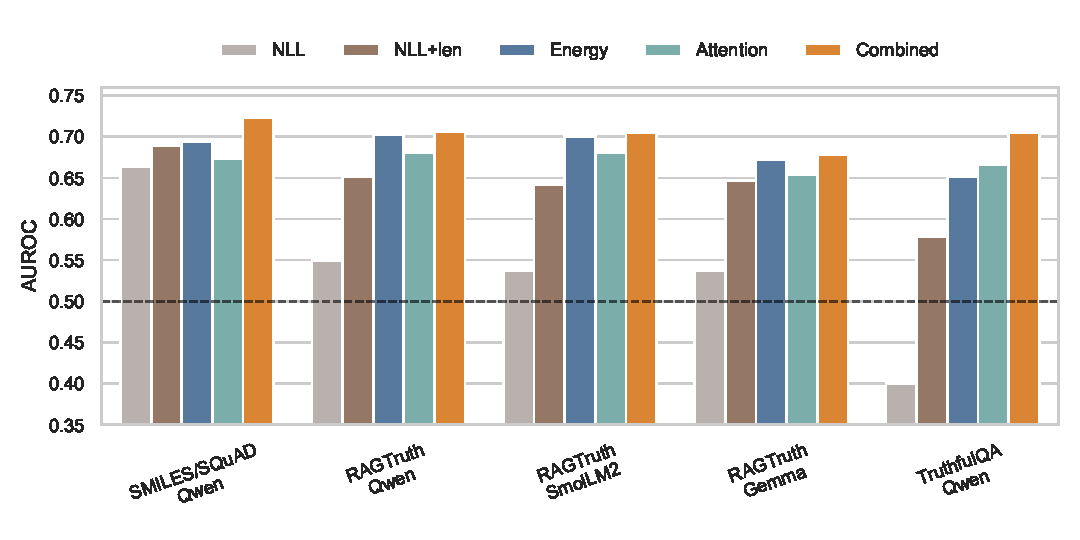
\includegraphics[width=0.95\linewidth]{figures/feature_family_auroc.pdf}
}{%
  \fbox{\parbox{0.85\linewidth}{Run \texttt{scripts/make\_final\_report\_figures.py} to generate
  \texttt{figures/feature\_family\_auroc.pdf}.}}
}
\caption{Feature-family comparison across datasets and models. The combined probe consistently
improves over response NLL; energy and attention features are most useful on RAGTruth.}
\label{fig:feature-family}
\end{figure}

\begin{figure}[t]
\centering
\IfFileExists{figures/best_auroc_by_run.pdf}{%
  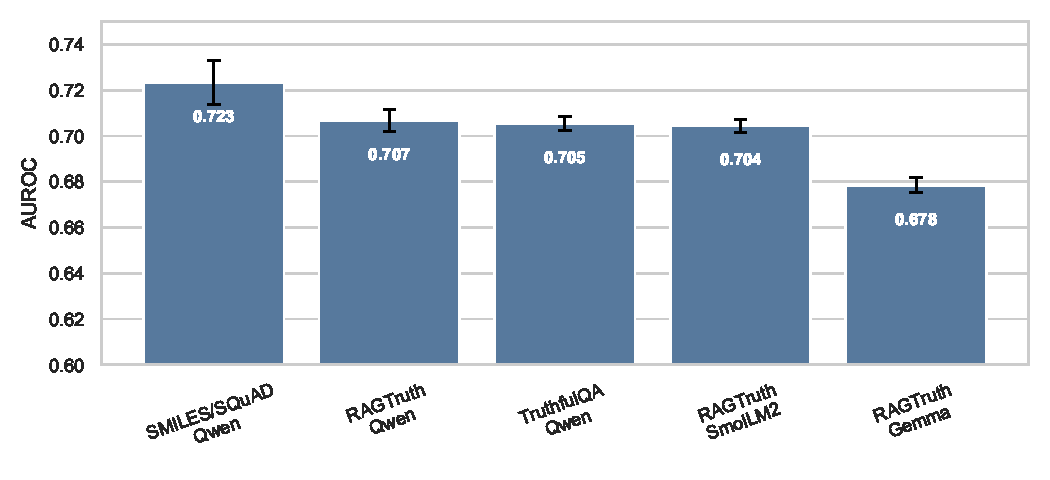
\includegraphics[width=0.92\linewidth]{figures/best_auroc_by_run.pdf}
}{%
  \fbox{\parbox{0.85\linewidth}{Run \texttt{scripts/make\_final\_report\_figures.py} to generate
  \texttt{figures/best\_auroc\_by\_run.pdf}.}}
}
\caption{Best combined AUROC across dataset/model settings. Error bars show standard deviation over
five cross-validation seeds.}
\label{fig:best-auroc}
\end{figure}

\subsection{Context-grounded hallucination}

The strongest context-grounded result is RAGTruth. In this setting, scalar response NLL is weak:
$0.550$ AUROC for Qwen and $0.537$ for SmolLM2. By contrast, per-layer Hopfield energy reaches
$0.703$ and $0.700$ respectively. This suggests that the Q/K geometry captures a support signal
that ordinary likelihood misses.

The result is not purely Qwen-specific. SmolLM2-360M gives almost the same RAGTruth AUROC as
Qwen2.5-0.5B. Gemma-3-1B is weaker, reaching $0.679$ with the best combined probe, but it still
improves over NLL+length. This weakens any claim that the method is architecture-invariant, but
supports the more modest claim that the signal is not limited to a single model family.

\subsection{Open-domain false answers}

TruthfulQA gives a different picture. The best combined probe still reaches $0.706$ AUROC, but
the scalar features behave differently. Raw response NLL has $0.400$ AUROC, and raw mean Hopfield
energy has $0.444$ AUROC in the single-run scalar evaluation. Negating the energy score improves
the scalar direction, while multifeature probes remain useful.

\begin{figure}[t]
\centering
\IfFileExists{figures/scalar_energy_direction.pdf}{%
  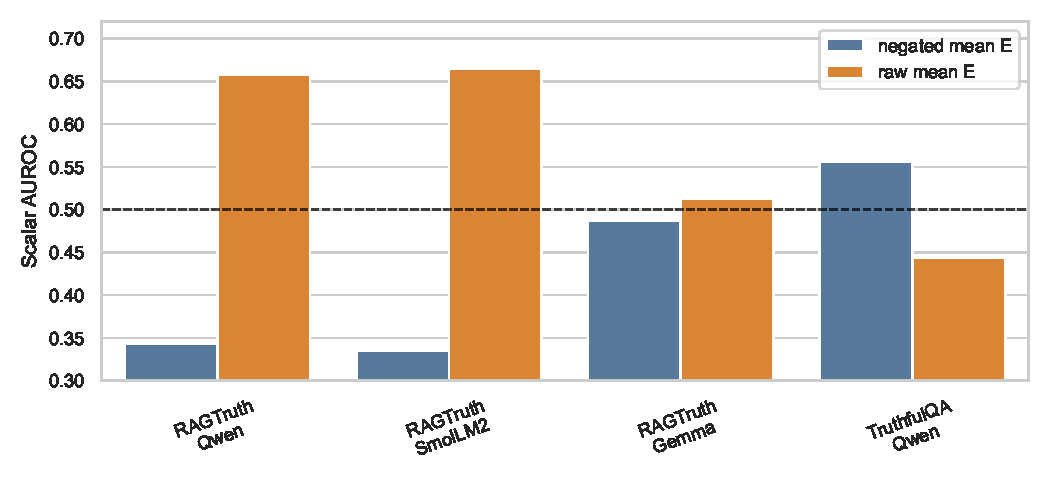
\includegraphics[width=0.92\linewidth]{figures/scalar_energy_direction.pdf}
}{%
  \fbox{\parbox{0.85\linewidth}{Run \texttt{scripts/make\_final\_report\_figures.py} to generate
  \texttt{figures/scalar\_energy\_direction.pdf}.}}
}
\caption{Scalar mean-energy AUROC differs by dataset. It is useful on RAGTruth for Qwen and
SmolLM2, weak on Gemma, and reverses direction on TruthfulQA.}
\label{fig:energy-direction}
\end{figure}

This result changes the interpretation of the method. A simple rule such as ``higher energy means
hallucination'' is too strong. The safer conclusion is that attention-derived Q/K features contain
factuality-relevant signal, but the sign and useful aggregation depend on the task.

\section{Discussion}

The results support the main hypothesis in a limited form. Attention-derived Hopfield energy and
prompt-grounding summaries contain hallucination signal beyond response likelihood. The strongest
evidence is RAGTruth, where energy-only per-layer probes outperform NLL+length on Qwen and
SmolLM2. The multi-seed standard deviations are small, so the effect is not just a lucky split.

At the same time, the study argues against an overly simple energy story. Energy is not a universal
scalar detector. On TruthfulQA, the scalar direction reverses, and Gemma shows weaker scalar
energy on RAGTruth than Qwen or SmolLM2. This points to a more cautious interpretation: Q/K
geometry is a useful representation for probing, not a standalone law of hallucination.

I also interpret the method as diagnostic rather than deployable. The classifier uses hidden
attention internals and requires access to model weights. It is therefore useful for understanding
model behavior and designing detectors, but it is not directly applicable to closed black-box
systems.

\section{Limitations}

The datasets are not identical in meaning. SMILES/SQuAD and RAGTruth evaluate context-grounded
support, while TruthfulQA evaluates correct versus incorrect answer candidates. These should not be
merged into one universal hallucination benchmark.

The model set is still small. Qwen, SmolLM2, and Gemma provide useful architectural diversity, but
the results may change for larger models, different layer choices, or models with substantially
different attention implementations.

The classifier is a probe trained on labels from the same dataset. Although cross-validation and
context-grouped splits reduce leakage concerns, the reported AUROC should not be interpreted as
out-of-domain deployment performance.

The method requires access to attention internals. It is not compatible with black-box APIs unless
the provider exposes equivalent intermediate states. It also adds extraction cost because Q/K tensors
must be processed for selected layers and response tokens.

Finally, the current features average over heads. This may hide a more localized mechanism. A future
analysis should study per-head contributions and layer sensitivity rather than only selected-layer
summaries.

\section{Conclusion}

This project tested whether attention-derived Hopfield energy and prompt-attention summaries contain
hallucination signal. The answer is positive but qualified. Across three datasets and three small
model families, simple probes over Q/K-derived features consistently improve over response
likelihood baselines. The strongest RAGTruth results transfer from Qwen2.5-0.5B to SmolLM2-360M,
and a weaker but positive result is observed for Gemma-3-1B.

The main scientific conclusion is not that Hopfield energy is a universal hallucination score. It is
that Q/K attention geometry provides a useful representation for factuality probing, while the scalar
energy direction depends on the hallucination type and architecture. This makes the result more
limited, but also more informative: internal attention geometry appears to encode support and
factuality signals, but these signals need careful calibration rather than a single fixed threshold.

\bibliographystyle{plainnat}
\bibliography{references}

\end{document}
